
\section{Introduction}
Electrical circuits are obviously both extremely useful and important to
modern society.  Society will expect you, as an engineer, to have a certain 
familiarity with the physical principles and phenomena responsible for making 
them function. You will obtain an understanding of these fundamentals in this 
course.  This lab examines circuits in which direct current flows. Future labs 
will examine the extended topic of alternating currents. 
  
We'll examine the concepts of voltage, current, and resistance; in particular,
how we can go about making measurements of them. In the process, we'll learn 
how to use the breadboard, an important device for experimenting with circuits.
We'll also take a look at the temperature dependence of resistance.  Finally,
we'll measure the internal resistance of a dry cell battery.

\section{Theory}

\subsection{References}

The concept of potential and potential difference is covered in Serway, 
Chapter~25 (Electric Potential).  The notions of electric current and 
resistance appear in Chapter~27 (Current \& Resistance), while DC 
circuits and Kirchoff's laws are introduced in Chapter~28 (DC Circuits). 
Since voltmeters and ammeters are the primary instruments we will use
to investigate circuits in the lab, we strongly suggest that you read over 
Section~28.5 (Electrical Instruments).  Other individual sections 
which will be particularly useful to us are: Section~27.3 (Resistance and 
Ohm's Law); Section~27.3 (Resistance and Temperature ), 
for a discussion of the temperature dependence of resistance; and 
Section~28.1 (Electromotive Force), for a discussion of the internal 
resistance of a battery. 
 
\subsection{Voltage, Current, and Resistance}

What is an electric circuit?  A succinct way of putting it is as follows:an 
electric circuit consists of a power source and a host of electrical 
components, all of which are connected together with wires.  The power source 
provides a force which makes electrons in the wire move.  These electrons in 
turn power the components of the circuit. After studying the concepts of 
voltage, current, and resistance, we'll be able to discuss power sources and 
resistors, so that we can understand the circuits we'll build with them. 

By now, you're familiar with the notion of electric potential.  A charge will
experience a force due to the electric fields of other charges around it.
The electric potential is defined as the potential energy per unit charge 
needed to move a charge (in the presence of these electric forces) from one 
point to another point.  It is important to remember that potential is defined
between two points. We can also talk about the potential at some point, but 
then we are referring to the potential between that point and some reference 
point, called the ``ground.''  Since the electric potential is defined 
everywhere in space, there will be a potential defined at every point of a 
circuit. We define {\it voltage} as the difference in the potential between 
two points in the circuit.  A battery, such as that in a car, is a power 
source which is said to provide ``12 volts.'' This means that the voltage
across the terminals of the battery is 12 V. 

If there is a potential difference between two points of a circuit, there is 
also a force on the electrons in the wire which causes them to move.  
{\it Current} is the rate at which this charge flows through the circuit,
{\it i.e.}, it is the amount of charge per unit time which passes a given 
point of the circuit. By {\it direct current}, or DC, we mean that the voltage 
and current values are steady; they do not vary in time. The circuits we'll be 
dealing with for our DC circuits will be composed of {\it conductors}, that is 
materials in which the electrons are free to move around.  It's pretty obvious 
that we wouldn't expect very much of a current to flow in a material that 
wasn't a good conductor. 

Given that a voltage induces a current, we can ask the question: what is the 
mathematical relationship between the two?  For most conductors, the 
relationship is one of direct proportionality.  Additionally, the voltage 
across a conductor always drops. Let's make all of this a bit clearer. 
Figure~\ref{fig:DC:voltdrop} shows part of a circuit containing a conductor 
which has a current $I$ flowing through it and a voltage $V$ across it 
(between points $a$ and $b$).  
We denote the voltage across the conductor by 
$$ V = V_a - V_b, $$
where $V_a$ is the potential difference between the point $a$ and ground (the 
common point referred to earlier) and $V_b$ is that between $b$ and ground.
By voltage drop, we mean that, in order for the current to flow in the
direction shown in the figure, the potential at $b$ must be less than that at
$a$, so that $V_a>V_b$, and $V$ is a positive number.
\begin{figure}[!htb]
\centering \epsfxsize=5cm 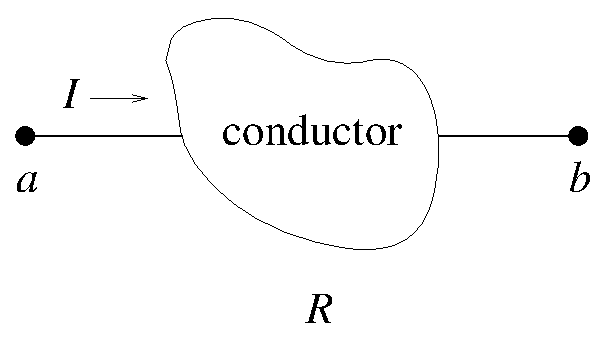
\includegraphics[scale=0.5]{2_dc/voltdrop.eps}
\caption{There is a voltage drop across a conductor.}
\label{fig:DC:voltdrop}
\end{figure}

The proportionality between the voltage and current is called Ohm's law, 
which we write as 
$$ \fbox{$ \displaystyle V=IR. $} $$
The constant of proportionality, $R$, is called the {\it resistance} of the 
conductor. The resistance depends on several factors. One is the size and 
shape of the conductor we're dealing with and another is called the 
{\it resistivity}, which is a property of the material and is independent of 
any particular shape. We will not examine this dependence of resistance on 
size and shape of the particular material in question. What we will examine is 
the temperature dependence of the resistivity of a material. If you pass enough
current through a conductor, you will raise the temperature of the conductor; 
a filament in a light bulb gets hot enough to glow.  At high enough 
temperatures, a conductor's resistivity, and therefore its resistance, will 
increase.  The voltage and current will no longer be proportional.  

\subsection{Diagrams and Meters}
Consider a simple DC circuit consisting of voltage sources and resistors.  A 
{\it resistor} is simply a conductor that has been constructed to have a 
particular resistance value (it's also made so that we can conveniently 
incorporate it into our circuits). The resistors are color-coded with the value
of their resistance. 
Before we go further, we should establish some conventions for our diagrams. 
Figure~\ref{fig:DC:voltsource} contains the schematic representations that we 
will use for voltage sources.  We also need some notation for resistors, 
voltmeters, and ammeters. 
Figure~\ref{fig:DC:schemdef} shows how these are represented.
\suppressfloats
\begin{figure}[!htb]
\centering \epsfxsize=8cm 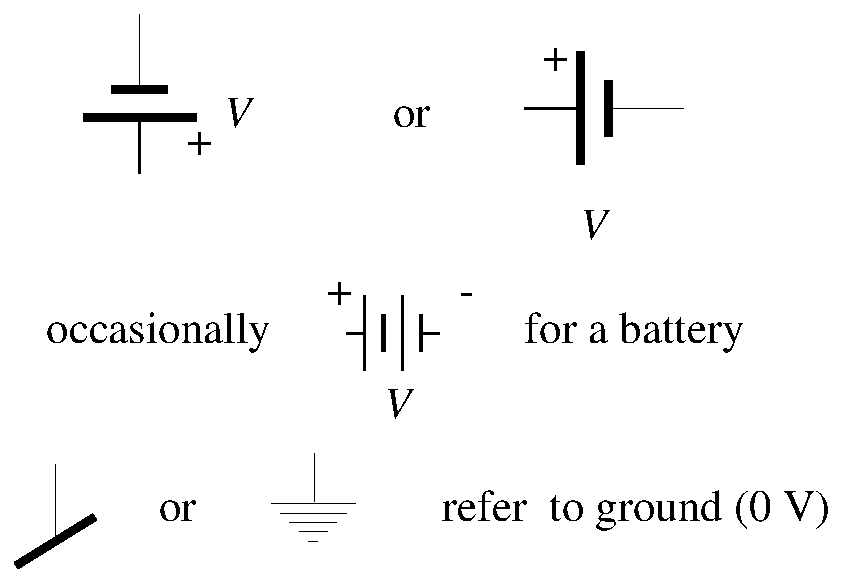
\includegraphics[scale=0.5]{2_dc/voltsource.eps}
\caption{Schematic symbols for voltage sources. $V$ refers to the voltage 
\hspace*{1cm} supplied. Don't confuse a ground with a regular voltage source.}
\label{fig:DC:voltsource}
\end{figure}

\begin{figure}[!htb]
\centering \epsfxsize=13cm 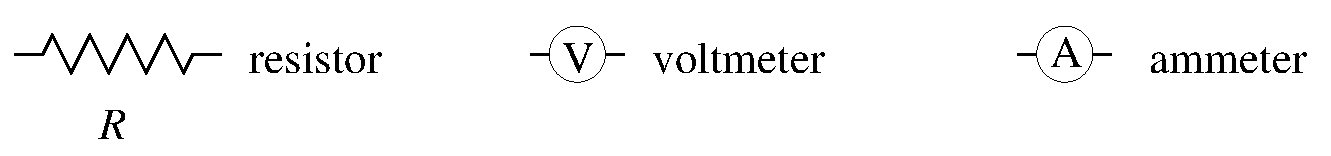
\includegraphics[scale=0.5]{2_dc/schemdef.eps}
\caption{Schematic symbols for circuit elements.}
\label{fig:DC:schemdef}
\end{figure}

\pagebreak
We will generally use two types of meters in our circuits, voltmeters and 
ammeters. Serway describes these, so we'll only concentrate on where they get 
connected to the circuit.  A voltmeter, as the name implies, measures voltage. 
The voltmeter is always connected {\it across} the part of the circuit that 
you want to measure the voltage across. In other words, it is connected in 
{\it parallel} with the part of the circuit you want to know the voltage 
across, as in Figure~\ref{fig:DC:voltmeter}.  
\begin{figure}[!htb]
\centering \epsfxsize=10cm 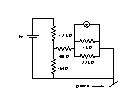
\includegraphics[scale=6]{2_dc/voltmeter.eps}
\caption{A voltmeter is always connected in parallel.}
\label{fig:DC:voltmeter}
\end{figure}

Remember that voltage is defined as the potential difference {\it between 
two points}.  One of these points could be a ground, but then you will need to 
connect the voltmeter between a point in the circuit and ground.  In any case,
if you've read the section on voltmeters in Serway, you'll remember that no 
current will flow through an ideal voltmeter, so it cannot be in series with 
the circuit. The voltmeter in the figure is in a position to measure the 
voltage across the parallel combination of the 1~k$\Omega$ and 2.2~k$\Omega$ 
resistors. An ammeter on the other hand, measures current, and it must be 
connected in {\it series} with the part of the circuit you want to know the 
current through, as in Figure~\ref{fig:DC:ammeter}. 
\begin{figure}[!htb]
\centering \epsfxsize=10cm 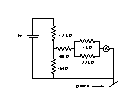
\includegraphics[scale=6]{2_dc/ammeter.eps}
\caption{An ammeter is always connected in series.}
\label{fig:DC:ammeter}
\end{figure}
This is because current is defined as the amount of charge which passes through
a {\it single point}.

\subsection{Voltage Sources}

The simplest DC circuit is a series combination of voltage sources as in 
Figure~\ref{fig:DC:voltseries}. 
\begin{figure}[htb]
\centering \epsfxsize=9cm 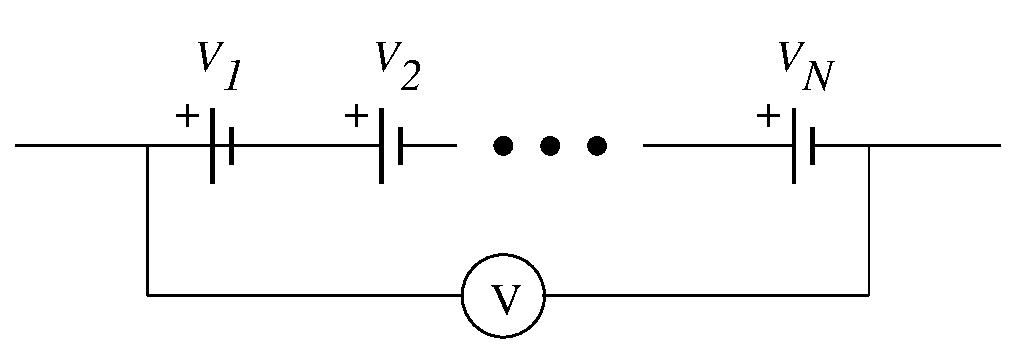
\includegraphics[scale=0.6]{2_dc/voltseries.eps}
\caption{A series of voltage sources.}
\label{fig:DC:voltseries}
\end{figure}
The total voltage across the circuit, which the voltmeter shown would display, 
comes from the rule that voltages in series add
$$
V = V_1 + V_2 \cdots + V_N.
$$
Let's apply this to some examples involving batteries.  In Figure 
\ref{fig:DC:battalign}, we connect two batteries with their voltages oriented 
in the same direction.  
\begin{figure}[htb]
\centering \epsfxsize=5cm 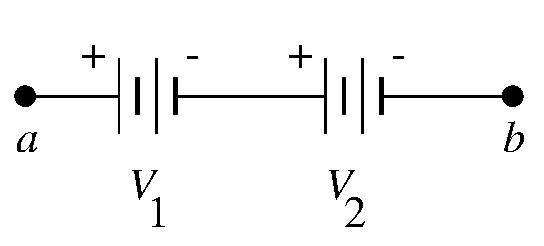
\includegraphics[scale=0.6]{2_dc/battalign.eps}
\caption{Two batteries in series.}
\label{fig:DC:battalign}
\end{figure}
The potential across the combination is
$$
V_{ab} = V_1 + V_2.
$$
In Figure~\ref{fig:DC:battopp}, two batteries have their voltages connected
in opposition.  
\begin{figure}[htb]
\centering \epsfxsize=5cm 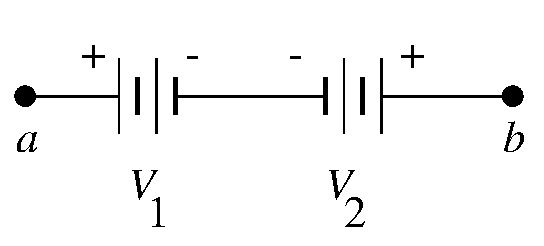
\includegraphics[scale=0.6]{2_dc/battopp.eps}
\caption{Two batteries in opposition.}
\label{fig:DC:battopp}
\end{figure}
The potential across the combination in this case is
$$
V_{ab} = V_1 + (-V_2)=V_1 - V_2.
$$
% There's too many floats hanging around, let's clear them 


We will not consider any circuits in which only voltage sources are connected 
in {\it parallel}, as shown in Fig~\ref{fig:DC:voltparallel}. 
\begin{figure}[htb]
\centering \epsfxsize=4cm 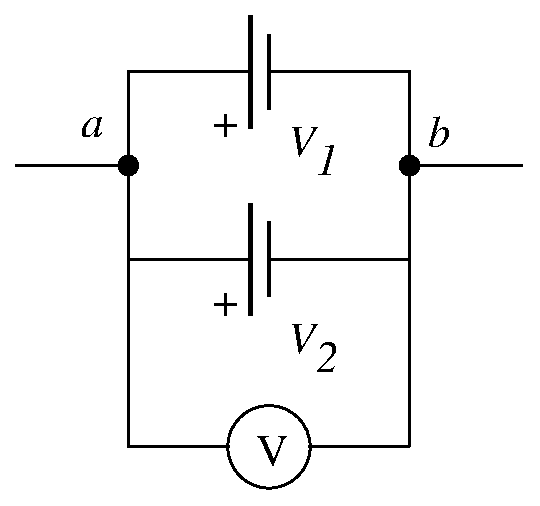
\includegraphics[scale=0.6]{2_dc/voltparallel.eps}
\caption{A parallel combination of voltage sources. We will never want to build
such a circuit.}
\label{fig:DC:voltparallel}
\end{figure}
The reason why we would not like to build such circuits is simple. Considering 
that the voltage source $V_1$ is connected between points $a$ and $b$ in 
Figure~\ref{fig:DC:voltparallel}, we would guess that the potential between $a$
and $b$ is $V_1$.  But since $V_2$ is also connected between points $a$ and 
$b$, the potential between them should be $V_2$.  Unless $V_1=V_2$, current 
will flow from one voltage source to another. Since most voltage sources do 
not like this, something will probably break!  Therefore, unless we want to 
destroy our voltage sources (and we don't!), we should be careful not to 
connect them in parallel.

\subsection{Series and Parallel Circuits with Resistors}

Resistors will also be an important part of the circuits we study.  In order
to deal with circuits with both voltage sources and resistors (and also any
other components, such as capacitors or inductors) we need to use two rules,
both attributed to Kirchoff.  The first is the {\it junction law: the sum of 
the currents passing into a point is equal to the sum of the currents leaving 
the point.} Such a point is illustrated in Figure~\ref{fig:DC:junction}, where 
arrows pointing into the point~$A$ indicate that the current is ingoing and 
the arrows pointing out mean the current is outgoing. 
\begin{figure}
\centering \epsfxsize=4cm 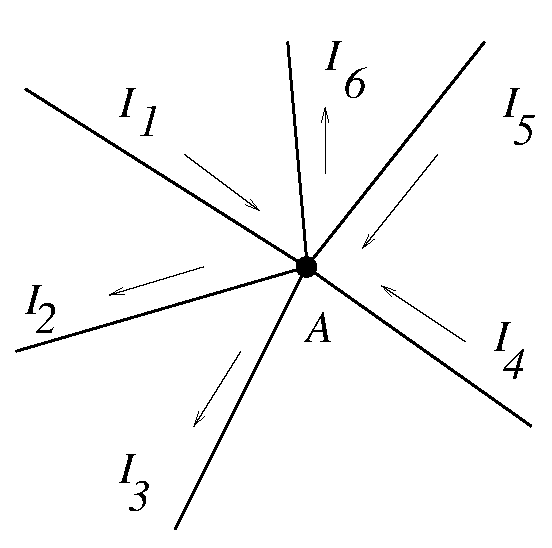
\includegraphics[scale=0.5]{2_dc/junction.eps}
\caption{Illustration of Kirchoff's junction rule.}
\label{fig:DC:junction}
\end{figure}
In the figure $I_1$, $I_4$, and $I_5$ are in going and $I_2$, $I_3$, and $I_6$ 
are outgoing, so that the junction rule tells us that
\begin{equation}
I_1+I_4+I_5=I_2+I_3+I_6. \label{eq:DC:junction}
\end{equation}  
The junction rule is simply a consequence of the principle of conservation of 
electric charge.  If a certain amount of charge passes into the point $A$ from
$I_1$, $I_4$, and $I_5$, it has to come out somewhere. It must leave $A$ 
through the combination of $I_2$, $I_3$, and $I_6$, leading to the conservation
statement (\ref{eq:DC:junction}). 

Before introducing the second rule, we need to understand the concept of a
voltage drop. Ohm's law tells us that, if we apply a potential $V$ across a
resistor of resistance $R$, the resistor will draw a current $I$ given by
$$
I=\frac{V}{R}.     
$$ 
Another way of looking at this comes from Figure~\ref{fig:DC:ohm}.
\begin{figure}[htb]
\centering \epsfxsize=4cm 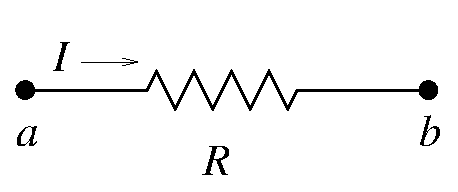
\includegraphics[scale=0.6]{2_dc/ohm.eps}
\caption{There is a voltage drop across a resistor.}
\label{fig:DC:ohm}
\end{figure}
If we know that a current $I$ is flowing through the resistor, then from Ohm's 
law, the potential difference from $a$ to $b$ is 
$$
V_b-V_a  = V_{ab} = -IR.
$$
Since $V_b$ is less than $V_a$, we say that there is a {\it voltage drop}
across the resistor.  The second rule now is the 
{\it circuit rule: between any two points in a circuit, the potential 
difference between the points is given by the sum of the potentials due to 
any sources between the points minus the sum of any voltage drops between the 
points.}  We can write this suggestively as an equation 
\begin{equation}
V_{ab} = \sum (\mbox{sources between $a$ and $b$}) 
- \sum (\mbox{drops between $a$ and $b$}). \label{eq:DC:circuitrule}
\end{equation}
We note that the circuit rule is usually expressed as a {\it loop} rule: 
{\it the sum of the voltage sources minus the sum of the drops around a closed 
loop is zero}.  We leave it as an exercise for the student to show that our 
rule reduces to this loop rule when applied to a closed loop. Note that the 
circuit law is a statement of energy conservation: the change in total energy 
(remember that voltage is a measure of potential energy) that occurs due to a 
charge moving from point $a$ to point $b$ is given by adding up all of the 
changes in its energy along its path.

Let us apply this circuit rule first to the series circuit in Figure 
\ref{fig:DC:series1}.  
\begin{figure}[htb]
\centering \epsfxsize=12cm 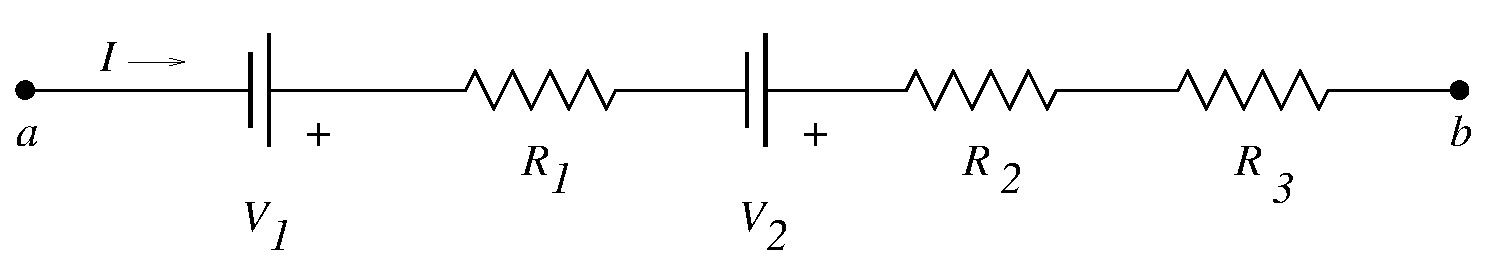
\includegraphics[scale=0.5]{2_dc/series1.eps}
\caption{A simple series circuit.}
\label{fig:DC:series1}
\end{figure}
We note that since everything is in series, there are no points where currents
branch out, so the junction rule tells us that the current through each of 
the elements has the same value $I$.  Applying the circuit rule 
(\ref{eq:DC:circuitrule}) to this we find
$$
V_{ab} = (V_1+V_2) - ( IR_1 + IR_2 + IR_3) = V_1+V_2 - I (R_1 + R_2 + R_3).
$$
We can also apply the circuit rule to a series combination of resistors, as
at the top of Figure~\ref{fig:DC:resistseries}.
Here the circuit rule tells us that
$$
V_{ab} = -I (R_1+R_2+\cdots+R_N).
$$
\begin{figure}[htb]
\centering \epsfxsize=10cm 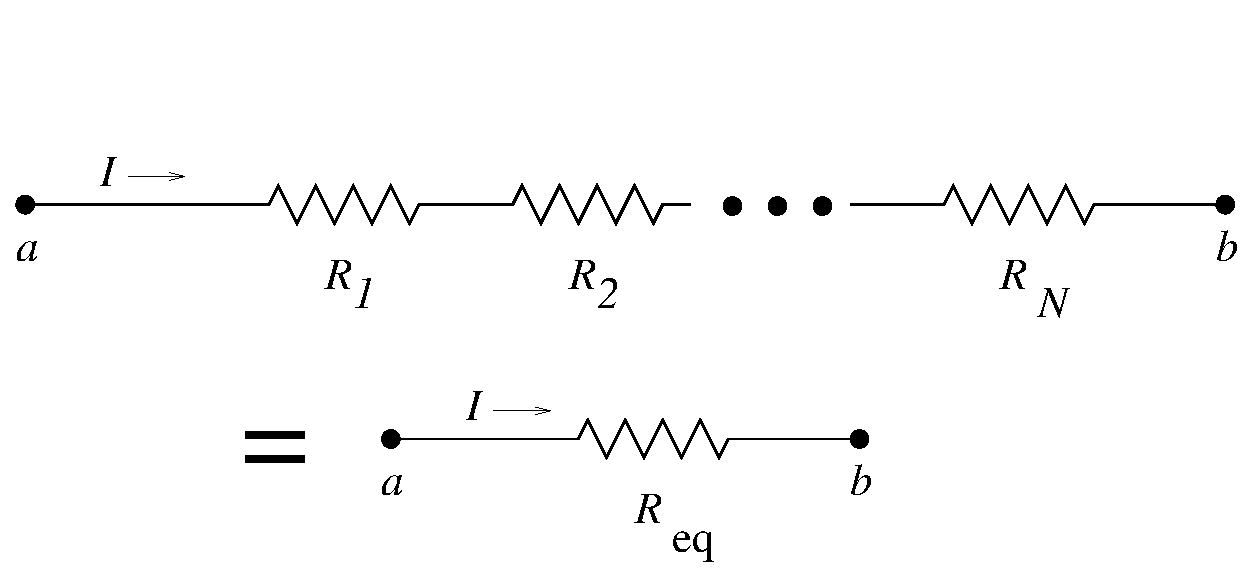
\includegraphics[scale=0.6]{2_dc/resistseries.eps}
\caption{Resistors in series and equivalent resistance.}
\label{fig:DC:resistseries}
\end{figure}
This series combination is the same as having a single resistor of resistance
(see the bottom of Figure~\ref{fig:DC:resistseries})
$$
R_{\mbox{eq}}=R_1+R_2+\cdots+R_N ~~~~~~~\mbox{(resistors in series)}.
$$
$R_{\mbox{eq}}$ is called the {\it equivalent resistance} of the series 
combination of resistors.  Note that the equivalent resistance of a combination
of resistors in series is always {\it greater} than the resistance of any of 
the individual resistors.

We also need to be able to deal with circuits in which some of the elements are
arranged in parallel. Since we have already seen that there are problems 
lurking in circuits for which voltage sources are in parallel, we will consider
circuits in which {\it only resistors} are in parallel. For concreteness, 
consider a specific example of such a circuit, shown in 
Figure~\ref{fig:DC:parallel1}.
\begin{figure}[htb]
\centering \epsfxsize=12cm 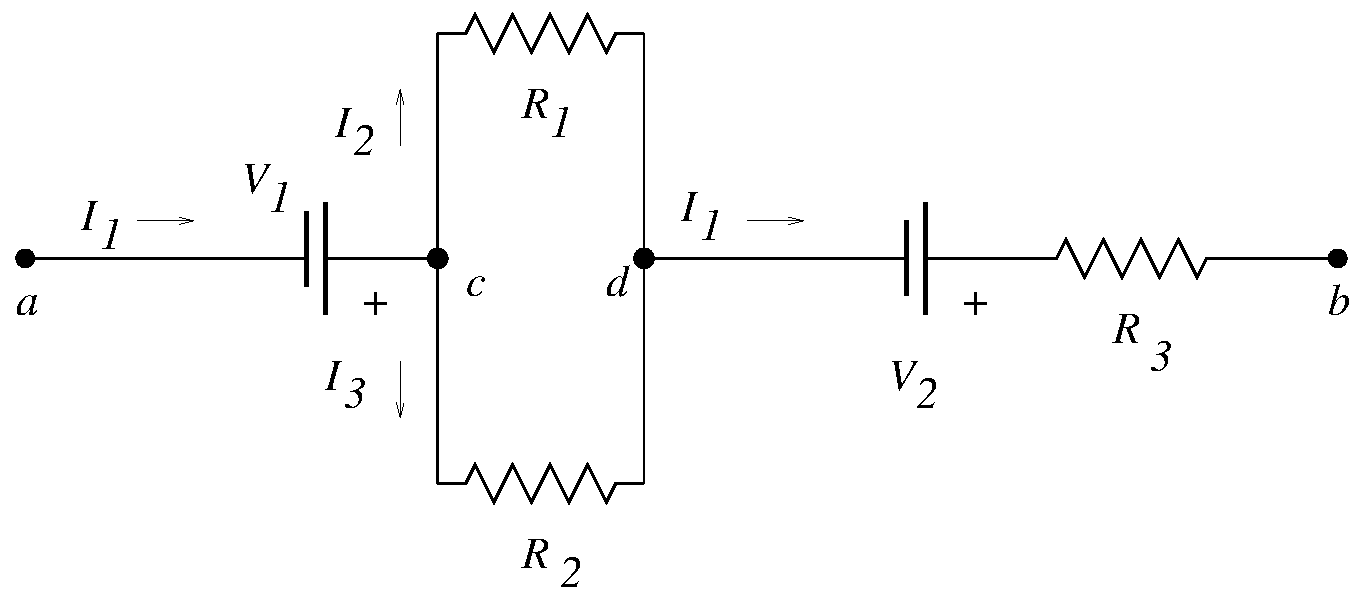
\includegraphics[scale=0.6]{2_dc/parallel1.eps}
\caption{A simple parallel circuit.}
\label{fig:DC:parallel1}
\end{figure}
This circuit is more complicated, since we have the junctions~$c$ and~$d$ where
we must apply the junction law. At~$c$, we have $I_1$ splitting up into $I_2$ 
and $I_3$, so that the junction rule tells us that $I_1=I_2+I_3$. At~$d$, we 
have $I_2$ and $I_3$ joining. Since $I_2+I_3=I_1$, the current leaving $d$ 
must be $I_1$.  Since we know how to apply the circuit rule to series circuits,
let's do the following. Note that whatever the voltage drop is across the 
parallel part of the circuit between $c$ and $d$ is, we can call it $V_{cd}$. 
Then the circuit rule gives us
\begin{equation}
V_{ab}= V_1 + V_{cd} + V_2 - I_1R_3.  \label{eq:DC:parallel1}
\end{equation}
%We subtract $V_{cd}$ since it is a voltage drop (only resistors contribute to it).
We now need to find out what $V_{cd}$ is.  For this purpose, we can 
simply concentrate on the relevant part of the circuit, shown in 
Figure~\ref{fig:DC:parallel2}.
\begin{figure}[htb]
\centering \epsfxsize=10cm 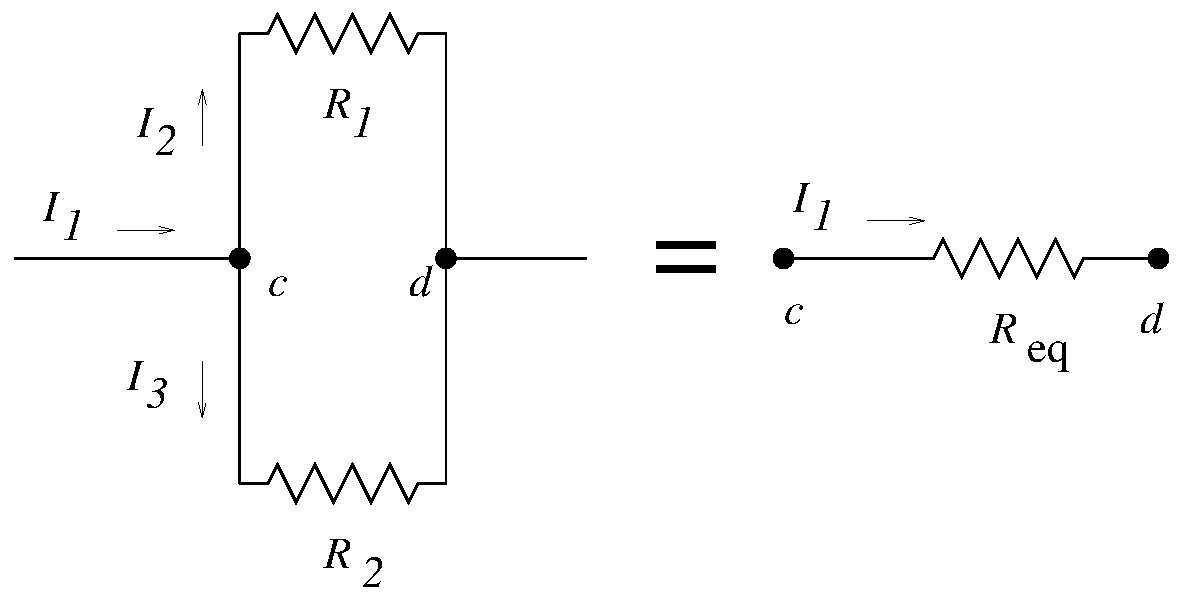
\includegraphics[scale=0.6]{2_dc/parallel2.eps}
\caption{The part of Figure~\ref{fig:DC:parallel1} contributing to $V_{cd}$.}
\label{fig:DC:parallel2}
\end{figure}
Note that we have introduced an equivalent resistor for this combination. Our
goal is to determine $R_{\mbox{eq}}$. From Ohm's law we find
$$
V_{cd}=-I_2R_1=-(I_1-I_2)R_2=-I_1R_{\mbox{eq}},
$$
where we have used $I_1=I_2+I_3$ to eliminate $I_3$ in the part from $R_2$.
These relations give us two useful equations
\begin{eqnarray*}
\frac{I_2}{I_1} &=& \frac{R_{\mbox{eq}}}{R_1} \\
R_{\mbox{eq}} &=& \left(1-\frac{I_2}{I_1}\right) R_2.
\end{eqnarray*}
Combining these, we find
$$
R_{\mbox{eq}} = \left(1- \frac{R_{\mbox{eq}}}{R_1} \right) R_2,
$$
so that, after some algebra, we have
$$
R_{\mbox{eq}} = \frac{R_1R_2}{R_1+R_2},
$$
or equivalently
\begin{equation}
\frac{1}{R_{\mbox{eq}}} = \frac{1}{R_1}+\frac{1}{R_2}.
\label{eq:DC:twoparallel}
\end{equation}
Therefore 
$$
V_{cd} = I_1 \frac{R_1R_2}{R_1+R_2}. 
$$
Then, from (\ref{eq:DC:parallel1}), for our original circuit we have
$$
V_{ab} = V_1+V_2- I_1 \left( \frac{R_1R_2}{R_1+R_2} +R_3 \right).
$$ 

The reasoning we used to deal with the parallel circuit example was a bit
roundabout, since we first had to learn how to approach the problem.  If we 
knew Equation~(\ref{eq:DC:twoparallel}) to begin with, we would have had much 
less to do. We can apply the same reasoning we gave the parallel combination 
of resistors in the example to a general parallel combination of resistors in
Figure~\ref{fig:DC:resistpar}.
\begin{figure}[htb]
\centering \epsfxsize=10cm 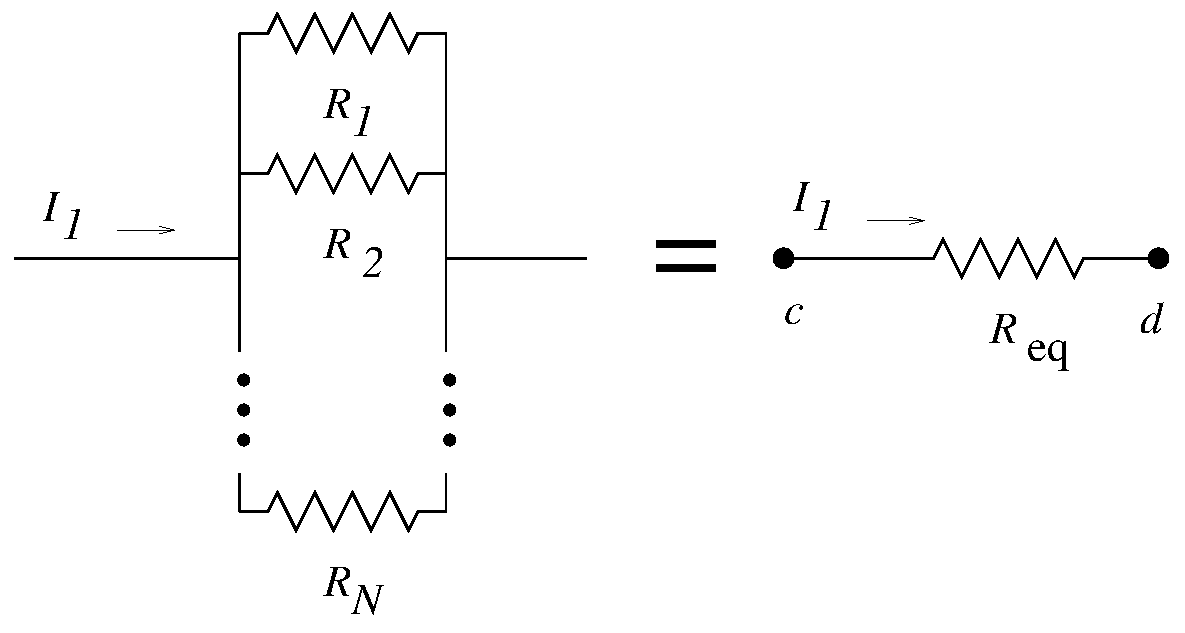
\includegraphics[scale=0.6]{2_dc/resistpar.eps}
\caption{Resistors in parallel.}
\label{fig:DC:resistpar}
\end{figure}
Since we already know what the equivalent resistance of two resistors in 
parallel is, we can approach this circuit by reducing a block of two resistors
down to a single equivalent resistor and then repeating the step until we're 
only left with one resistor; see Figure~\ref{fig:DC:parallelred}.
\begin{figure}[htb]
\centering \epsfxsize=14cm 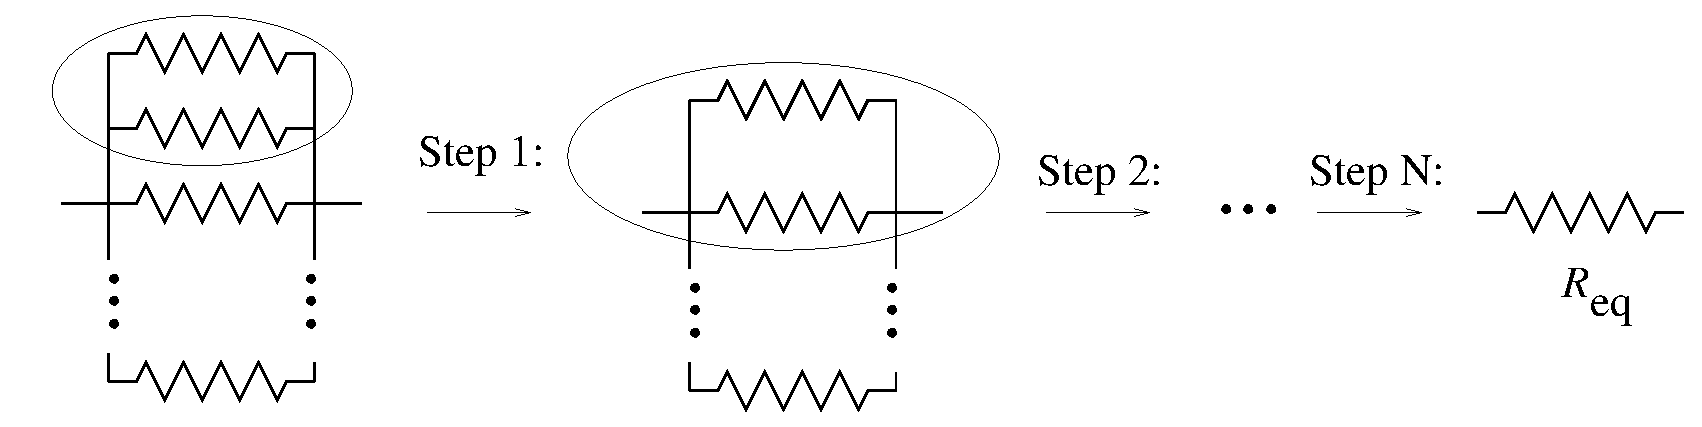
\includegraphics[scale=0.5]{2_dc/parallelred.eps}
\caption{The steps used to obtain Equation~(\ref{eq:DC:resparallel}).}
\label{fig:DC:parallelred}
\end{figure}
You might label the resistors with resistance values and work out a few steps 
of the algebra to convince yourself that the general result for resistors in 
parallel is 
\begin{equation}
\frac{1}{R_{\mbox{eq}}} = \frac{1}{R_1} + \frac{1}{R_2}+\cdots +\frac{1}{R_N}
~~~~~~~\mbox{(resistors in parallel)}.  \label{eq:DC:resparallel}
\end{equation}
In contrast with the situation of resistors in series, the equivalent 
resistance of a parallel combination of resistors is always {\it less} than
any of the individual resistances.  Knowing these rules of thumb can come in 
handy when your circuit requires a resistance that isn't among the values
of the resistors you have available to you.  You'll be able to build series and
parallel combinations of the resistors you do have to get an equivalent 
resistance that will be fairly close to what you need.


With the junction and circuit rules and the rules for adding resistors in 
series and in parallel, we can approach circuits by using equivalent resistors 
to reduce the circuit in steps, as in Figure~\ref{fig:DC:resistreduce}. (For 
simplicity we consider a circuit with only resistors.)  
A good exercise would be to calculate the equivalent resistances needed in each
step of Figure~\ref{fig:DC:resistreduce}.  
\begin{figure}[htb]
\centering \epsfxsize=9cm 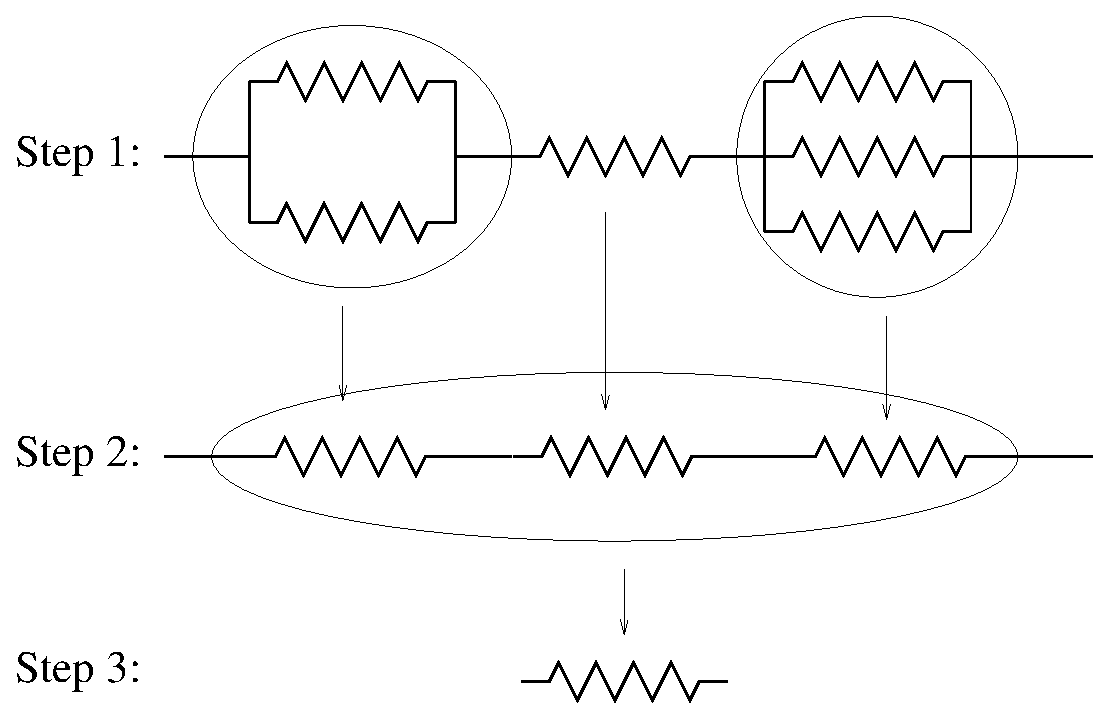
\includegraphics[scale=0.6]{2_dc/resistreduce.eps}
\caption{Reduce the resistor combinations in terms of equivalent resistors.}
\label{fig:DC:resistreduce}
\end{figure}

\subsection{The Color Code for Resistors}

Colored bands are drawn on the resistors to denote the resistance, as 
depicted in Figure~\ref{fig:DC:colorcode}. 
For a figure with color, see Figure 27.7 on page 747 of Serway.
To read the color code of a resistor, pick up the resistor and identify the
first band. The first band is the band closest to the outside of the resistor 
that is a color other than gold or silver.  If there are no gold or silver 
bands, the colored bands will be clearly off-center and the first band is that 
closest to the outside of the resistor.  Identify the number associated
with the first band in Table~\ref{tab:DC:colorcode}. 
This is the first digit of the resistance value of the resistor.  The color of 
the second band refers to the second digit of the resistance. The color of the 
third band refers to the power of ten you need to multiply the two digits by 
to get the resistance in Ohms. A fourth band that is gold or silver refers to 
the tolerance or precision with which you can trust the nominal value of 
resistance obtained from the color code. Resistors without a fourth band have
a tolerance of $\pm 20$\%.  On rare occasions a resistor will have a fifth 
colored band, which refers to a military specification of reliability. We will 
not worry about this rare option, but take note of it so that we do not 
confuse this band with the most important first band. \\

\begin{figure}[!htb]
\centering \epsfxsize=9cm 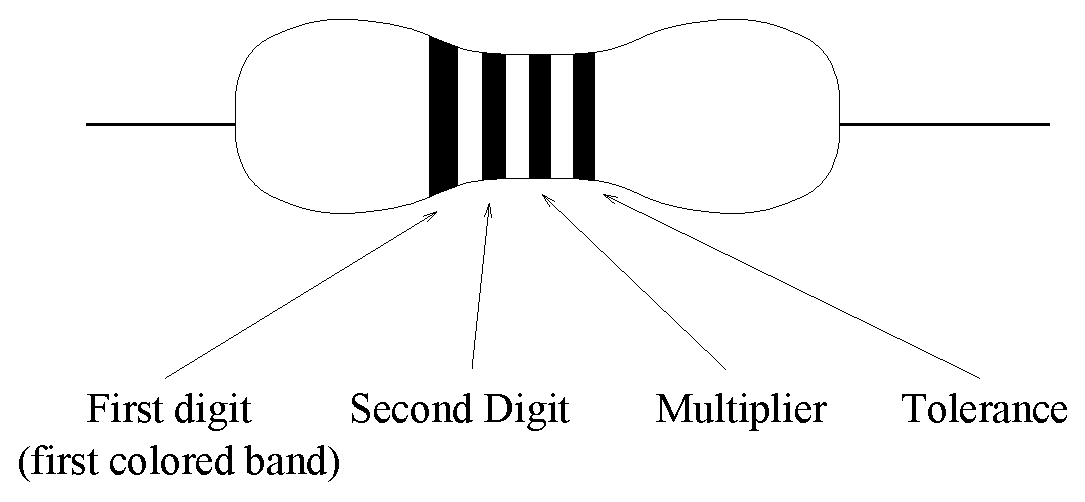
\includegraphics[scale=0.4]{2_dc/resistor.eps}
\caption{Resistors are color-coded with their resistance value.}
\label{fig:DC:colorcode}
\end{figure}
\begin{table}[htb]
\begin{center}
\begin{tabular}{|l|c|c|c|}
\hline
Color & Number & Multiplier & Tolerance (\%) \\
\hline
Black     & 0 & 1      &      \\
Brown     & 1 & $10^1$ &      \\
Red       & 2 & $10^2$ &      \\
Orange    & 3 & $10^3$ &      \\
Yellow    & 4 & $10^4$ &      \\
Green     & 5 & $10^5$ &      \\
Blue      & 6 & $10^6$ &      \\
Violet    & 7 & $10^7$ &      \\
Gray      & 8 & $10^8$ &      \\
White     & 9 & $10^9$ &      \\
Gold      &   &        & 5\%  \\
Silver    &   &        & 10\% \\
Colorless &   &        & 20\% \\
\hline
\end{tabular}
\end{center}
\caption{The resistor color code.}
\label{tab:DC:colorcode}
\end{table}

Some examples are in order.\\
\begin{tabular}{cccccc}
Colors & First & Second & Multiplier & Resistance & Tolerance \\
& Digit & Digit & & & \\
Yellow-Orange-Brown-Gold & 4 & 3 & 10 & 430  $\Omega$ & $\pm 5$\%  \\
%& & & & & \\
Red-Red-Red   & 2 & 2 & $10^2$ & 2.2 k$\Omega$ & $\pm 20$\% 
\end{tabular}

\section{Apparatus}

\subsection{The Multimeter}

The multimeter, illustrated in Figure~\ref{fig:DC:multimeter}, serves three 
functions: voltmeter, ammeter, and ohmmeter. 
\begin{figure}[htb]
\centering \epsfxsize=6cm 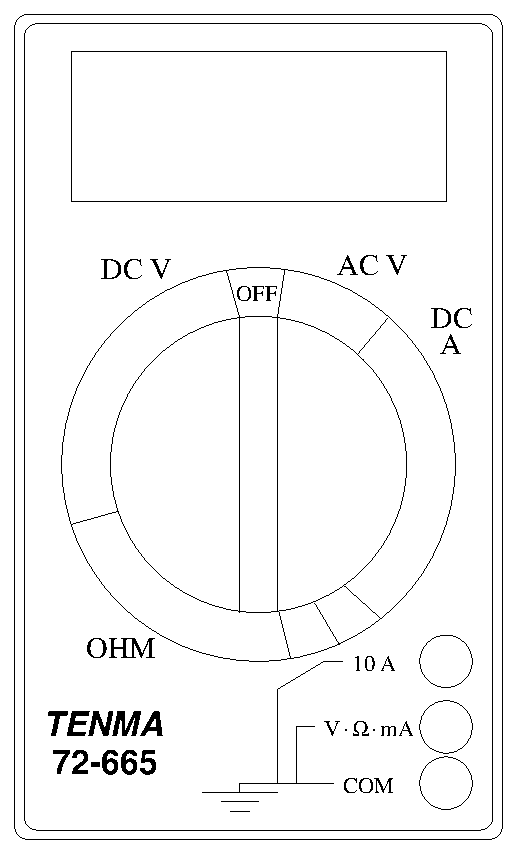
\includegraphics[scale=0.7]{2_dc/multimeter.eps}
\caption{The multimeter.}
\label{fig:DC:multimeter}
\end{figure}
The {\it ranges} for each setting indicate the maximum value of the particular
quantity (voltage, current, or resistance) that can be measured in that 
setting.  For example, the 200~mA setting will allow you to measure a current
that is between 0 and 200~mA. If you attempt to measure a value higher than the
maximum, the display will read ``1.''  When this happens, it indicates that you
need to try a larger scale.  The {\it uncertainty} in a measurement with
the multimeter is a $\pm 1$ in the last decimal place; for example, if you read
a current of 98~mA, then the uncertainty is $\pm 1$~mA, so you should write
down the measurement as $98\pm 1$~mA.  You should notice that a lower scale
setting will often give you an extra significant figure (as long as the scale 
isn't too low), so that you can get the greatest precision in a measurement by 
using the smallest scale setting possible.  For example, a lower scale setting
with the current from our last example might give us $98.3\pm 0.1$~mA, which 
has a relative uncertainty of 0.1\%, rather than the 1\% uncertainty in the 
first measurement. If it appears from the value of a measurement that you can 
use a smaller scale setting, and therefore improve the precision of a 
measurement, then be sure you do so.

The multimeter probes are color-coded: red for positive and black for ground.
Always connect the red probe to the V$\cdot\Omega\cdot$mA port on the 
multimeter and the black probe to that marked COM. If you are using an 
ohmmeter setting to measure resistance, the order in which you connect the 
probes {\it to the circuit} will not matter.  When set as a voltmeter, the 
value of voltage read will be positive or negative, depending on the sign of 
the potential across the part of the circuit you are trying to measure.  It is 
therefore a good idea to make a note of the order in which you connected your 
probes or, in a simple circuit, to follow a convention of always placing the 
black probe closest to ground, since the sign of the voltage is an important 
part of your measurement.  The order is crucial when using the multimeter as 
an ammeter.  If you do not have the current flowing from {\it red to black}, 
the ammeter will not allow the current to flow and you risk {\it damaging} the 
multimeter. Disconnect the ammeter immediately if you believe you have the 
connection wrong; then reexamine the circuit to determine the correct 
orientation. 

\subsection{The Power Supply}
 
The power supply we'll be using is illustrated in 
Figure~\ref{fig:DC:powersupply}.
It can supply a DC signal at a fixed voltage and can limit the current drawn
by the circuit; there are both fine and coarse adjustment knobs and there are
meters to display the voltage and current settings.  We will make all of our 
voltage and current measurements with the multimeter, so use the values 
displayed on the power supply's meters only as a reference.  The supply 
contacts on the front of the unit are marked $+$~(for positive), GND~(for 
ground), and $-$~(for negative); our units have had the $-$~and 
GND~connections wired together so that they are both at ground. Make your 
connections to the $+$ and GND contacts. 
\begin{figure}[!htb]
\centering \epsfxsize=8cm 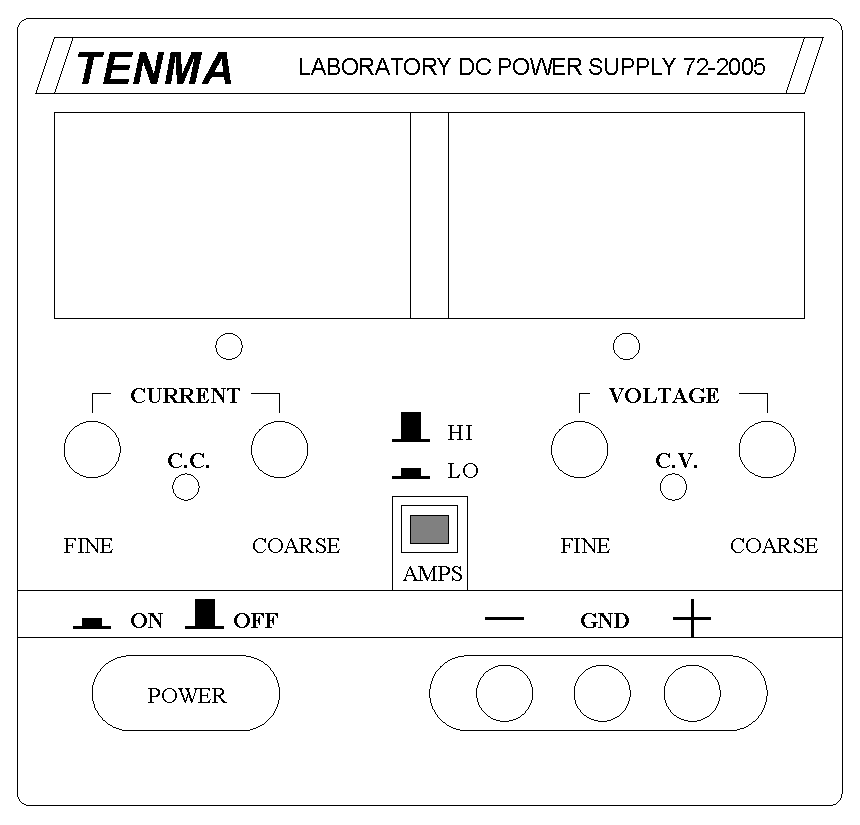
\includegraphics[scale=0.6]{2_dc/powersupply.eps} 
\caption{The power supply.}
\label{fig:DC:powersupply}
\end{figure}

\subsection{The Breadboard}

The breadboard, illustrated in Figure~\ref{fig:DC:breadboard}, conveniently 
provides power and electrical connections for our circuits.   
\begin{figure}[!htb]
\centering \epsfysize=17cm 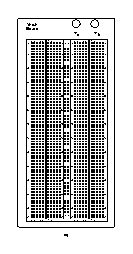
\includegraphics[scale=4]{2_dc/breadboard.eps} 
\hspace*{1cm} \epsfysize=16cm 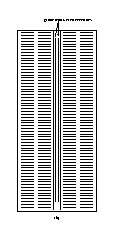
\includegraphics[scale=4]{2_dc/backboard.eps} 
\caption{(a) The breadboard. (b) The wiring connections on the board.}
\label{fig:DC:breadboard}
\end{figure}
Figure~\ref{fig:DC:breadboard}b shows the detail of the wiring connections on
the board. The power and ground connections are contiguous, while many short
``wire'' sections are provided for circuit building.  The best way to learn how
to use the breadboard is to just start building circuits, but to better 
prepare you, we'll provide an example of how to use the breadboard to power a 
resistor. 
We want to build the circuit shown in Figure~\ref{fig:DC:exampleboard}a.
\begin{figure}[!htb]
\centering \epsfysize=16cm 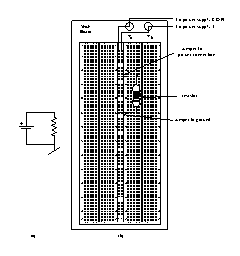
\includegraphics[scale=4]{2_dc/exampleboard.eps} 
\caption{(a) The circuit schematic. (b) The necessary connections on the 
board.}
\label{fig:DC:exampleboard}
\end{figure}
The necessary connections are shown in Figure~\ref{fig:DC:exampleboard}b. We 
start by connecting the power supply to the $V_a$ and $V_b$ connections on the 
board; the $V_a$ connection will be the ground and is also connected to the
A~ground line on the board, the $V_b$ connection will be the ``hot'' connection
and will be connected to the power line on the board.  A small jumper wire
connects the power line to one of the wire sections.  The resistor is plugged
between this section and another section which is jumped to ground. Carefully
compare Figure~\ref{fig:DC:exampleboard}b and Figure~\ref{fig:DC:breadboard}b,
so that you understand how other connections should be made.  A good exercise
would be to make a rough sketch of the board outline for all of the circuits
listed in the Procedure and Analysis section below.  You'll need to build them
when you come into lab anyway; why not prepare? A good quiz question would be 
to give you a circuit and a sketch of the board; you'd draw the jumper and
element connections needed on the sketch\ldots 
\vfill
\pagebreak
$$
$$
\vfill
\clearpage
\newpage

%  Label worksheets by \thechapter.W1
\renewcommand{\thesection}{\thechapter.W1}

\section{DC Circuits Part I Worksheet}

{\bf \Large Name:}~ \rule{5cm}{.1mm}~~~~~~~
{\bf \Large Day/Time:}~\rule{3cm}{.1mm}\\
{\bf \Large Partner's Name:}~\rule{6cm}{.1mm}\\

\noindent All measurements with the multimeter should include {\it units} and 
{\it uncertainty}. In general, you should turn down the voltage to zero 
on the power supply whenever you rearrange the circuit on the breadboard. 
Record your observations in the spaces provided as you proceed through this
worksheet.  Be sure to check off each item on
the check list included before you leave lab.

\subsection{In-Lab Procedure}

\subsubsection{Batteries in Series and Opposition}

Measure the voltage supplied by each of the batteries, and enter those values
into Table~\ref{tab:DC:battseries}.  Take care to 
distinguish between the batteries once you've made your measurements. 
Calculate the expected voltage 
value you would read on a voltmeter with uncertainties. First if they were in series 
and second if they were in opposition.  {\bf Space is provided here for the 
calculation.} \\
\vskip\baselineskip
\vskip\baselineskip
\vskip\baselineskip 
\noindent Enter these values into the spaces titled ``Expected Value'' in 
Table~\ref{tab:DC:battseries}.  Connect 
the batteries in series as in Figure~\ref{fig:DC:procbatt}a and measure the voltage 
across the combination entering your data into Table~\ref{tab:DC:battseries}.
\begin{figure}[htb]
\centering \epsfxsize=10cm 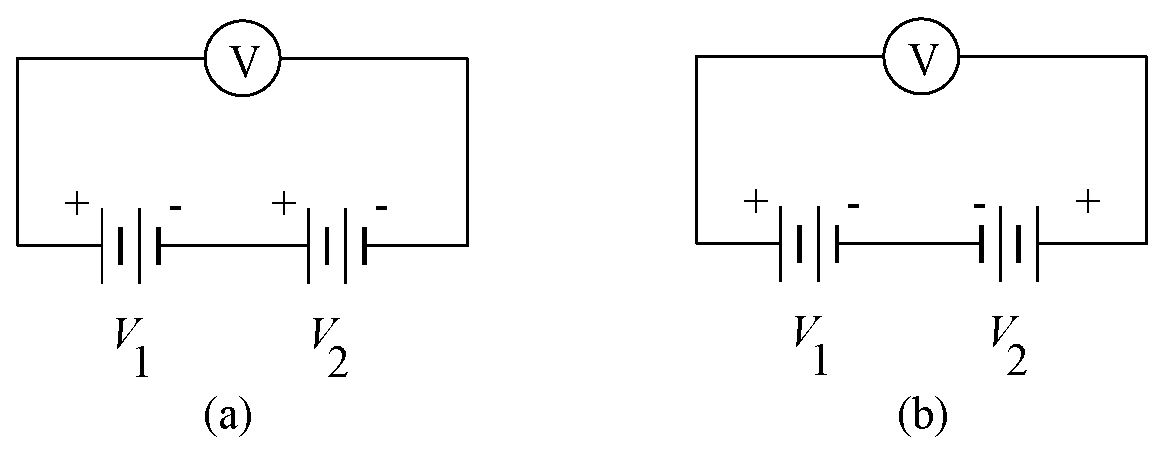
\includegraphics[scale=0.7]{2_dc/procbatt.eps}
\caption{Batteries in Series and Opposition.}
\label{fig:DC:procbatt}
\end{figure}
\noindent Now connect the 
batteries in opposition, as in Figure~\ref{fig:DC:procbatt}b.  
Measure the voltage across the combination entering your data 
once again into Table~\ref{tab:DC:battseries}.

\begin{table}[!htb]
\begin{center}
\begin{tabular}{|c|c|}
\hline
Battery 1 Voltage, $V_1$ & Battery 2 Voltage, $V_2$  \\ 
\hline
\hspace*{5cm} & \hspace*{5cm}\\
& \\
\hline
\hline
Voltage in Series, $V_{s,\rm meas}$ & Expected Value, $V_{s,\rm exp}$\\
\hline
& \\
& \\
\hline
Voltage in Opposition, $V_{o,\rm meas}$ & Expected Value, $V_{o,\rm exp}$\\
\hline
& \\
& \\
\hline
\end{tabular}
\end{center}
\caption{Voltage measurements.}
\label{tab:DC:battseries}
\end{table}

\subsubsection{Resistance Measurement}
\label{sec:DC:resist}

Pick two resistors and use the color code to determine their nominal resistance
and tolerance. Use the ohmmeter setting of the multimeter to measure their
resistance.
Note that you are taking {\bf 3} measurements of
{\bf 2} resistors.  First you use the color code, next the ohmmeter, and 
finally the circuit.  Using the circuit means you will make 2 measurements:
you will measure voltage and current across the resistor.  When you measure
resistance in the circuit, disconnect the power supply.  When you measure
{\bf current, place the ammeter IN SERIES} as dictates 
Figure~\ref{fig:DC:procresist}. \\   

\noindent The set-up for the circuit to measure resistance is outlined 
in Figure~\ref{fig:DC:procresist}.  
Begin by disconnecting the batteries and connecting the {\bf power source}
to the breadboard. Set the power source 
to a voltage of approximately 3 V. Pick one of your resistors and build the 
circuit in Figure~\ref{fig:DC:procresist}. You will need to include jumper 
wires so that you can make the necessary connection for the current 
measurement.  Measure the voltage across and the current through the resistor
({\bf in series}).
Use Ohm's law to calculate the resistance with uncertainty.  Repeat the
measurement with your other resistor.   \\

\begin{figure}[htb]
\centering \epsfxsize=6cm 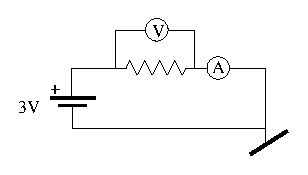
\includegraphics[scale=1.5]{2_dc/procresist.eps}
\caption{Circuit used to measure resistance.}
\label{fig:DC:procresist}
\end{figure} 

\noindent Enter the color code resistance value (not the colors), the ohmmeter reading,
the voltage and current readings, and the Ohm's law resistance  with 
uncertainties into Table~\ref{tab:DC:resistmeas}.
\begin{table}[h]
\begin{center}
\begin{tabular}{|c|c|c|}
\hline
\multicolumn{3}{|c|}{Resistor 1} \\
\hline 
Color Code, $R_{1,1}$ & Ohmmeter, $R_{1,2}$ & Leave Blank\\ 
\hline
\hspace*{3cm} & \hspace*{3cm} & \hspace*{3cm} \\ 
& &  \\ 
\hline
Voltage, $V_1$ & Current, $I_1$ & Ohm's Law Resistance, $R_{1,3}$ \\
\hline
& &  \\
& &  \\
\hline
\hline
\multicolumn{3}{|c|}{Resistor 2} \\
\hline 
Color Code, $R_{2,1}$ & Ohmmeter, $R_{2,2}$ & Leave Blank\\ 
\hline
\hspace*{3cm} & \hspace*{3cm} & \hspace*{3cm} \\ 
& &  \\ 
\hline
Voltage, $V_2$ & Current, $I_2$ & Ohm's Law Resistance, $R_{2,3}$ \\
\hline
& &  \\
& &  \\
\hline
\end{tabular}
\end{center}
\caption{Resistance measurements.}
\label{tab:DC:resistmeas}
\end{table}


\subsubsection{Resistors in Series and Parallel}

{\bf Using the same resistors as above}, build the series and 
parallel circuits in
Figure~\ref{fig:DC:procserpar}.  
\begin{figure}[htb]
\centering \epsfxsize=14cm 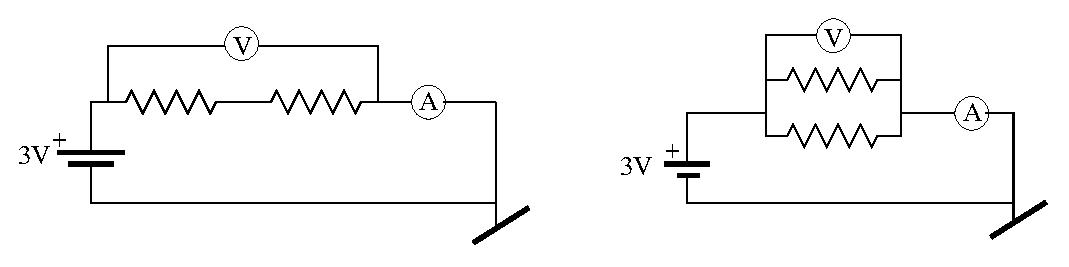
\includegraphics[scale=0.7]{2_dc/procserpar.eps}
\caption{Series and parallel resistance measurements.}
\label{fig:DC:procserpar}
\end{figure}
Note that you now have 
chosen {\bf 2} resistors
and measured their resistances in {\bf 3} ways. In this section, you will
use those 2 resistors to build {\bf 2} circuits, one in series and one in
parallel.  You are doing {\bf 2 circuits} and will need to collect data 
for each circuit. 

\noindent
Calculate the nominal resistances of the new circuits and their errors from the nominal values in Table~\ref{tab:DC:resistmeas}. Write the expressions here, and then enter the numerical values and uncertainties into the Color Code section in Table~\ref{tab:DC:SeriesParallelRmeas}.\\
\vspace*{4cm}

\noindent Measure with the ohmmeter the new circuits' resistance, entering the data into
Table~\ref{tab:DC:SeriesParallelRmeas}. Measure the  voltage and the current
for the 2 circuits, once again being careful to place the {\bf ammeter
in SERIES} with the resistors.  Enter the voltage, current, and Ohm's law 
resistance into Table~\ref{tab:DC:SeriesParallelRmeas}. \\

\begin{table}[htb]
\begin{center}
\begin{tabular}{|c|c|c|}
\hline
\multicolumn{3}{|c|}{Series Resistors} \\
\hline 
Color Code, $R_{s,1}$ & Ohmmeter, $R_{s,2}$ & Leave Blank\\ 
\hline
\hspace*{3cm} & \hspace*{3cm} & \hspace*{3cm} \\ 
& &  \\ 
\hline
Voltage, $V_s$ & Current, $I_s$ & Ohm's Law Resistance, $R_{s,3}$ \\
\hline
& &  \\
& &  \\
\hline
\hline
\multicolumn{3}{|c|}{Parallel Resistors} \\
\hline 
Color Code, $R_{p,1}$ & Ohmmeter, $R_{p,2}$ & Leave Blank \\ 
\hline
\hspace*{3cm} & \hspace*{3cm} & \hspace*{3cm} \\ 
& &  \\ 
\hline
Voltage, $V_p$ & Current, $I_p$ & Ohm's Law Resistance, $R_{p,3}$ \\
\hline
& &  \\
& &  \\
\hline
\end{tabular}
\end{center}
\caption{Series and parallel resistance measurements.}
\label{tab:DC:SeriesParallelRmeas}
\end{table}

\subsection{Part I Pre-Classroom Check List}
\noindent This check list is intended to be a guide for 
you to prepare yourself 
for the classroom work.  You cannot come back to lab during this hour,
collaborate with colleagues, nor hand in the worksheet late.  Make sure
you have completed everything.  
\vskip \baselineskip
\noindent {\bf Pre-classroom Check List}  
\vskip\baselineskip
\noindent $\bigcirc$ \hspace*{1cm} Table~\ref{tab:DC:battseries} completed with units and uncertainties\\
$\bigcirc$ \hspace*{1cm} Table~\ref{tab:DC:resistmeas} completed with units and uncertainties\\
$\bigcirc$ \hspace*{1cm} Table~\ref{tab:DC:SeriesParallelRmeas} completed with units and uncertainties\\


\subsection{In-Classroom Calculations \& Analysis}

\noindent
\subsubsection{Batteries in Series and Opposition}

\noindent Using Table~\ref{tab:DC:battseries}, compare your measured results 
with those that you calculated as expected.
Do the values match within uncertainty? Refer to § \ref{sec:intro:agreement}. \\
\vspace*{2cm}%neel

\subsubsection{Resistance Measurement}
\noindent For each resistor in Table~\ref{tab:DC:resistmeas}, you have three 
values of resistance: nominal (color 
code), ohmmeter, and Ohm's Law.  Do all the measured (ohmmeter and Ohm's
Law) values agree with the nominal (color code) 
value within uncertainty for both resistors? \\
\vspace*{4cm}\\
\noindent Calculate the average resistance of each resistor using 
equation~(\ref{eq:intro:average}) and the standard deviation with 
equation~(\ref{eq:intro:standdev}).\\  
\vspace*{4cm}\\
\noindent Discuss the validity of your results using the above calculations,
i.e. what values make sense and why.  \\


\subsubsection{Resistors in Series and Parallel}

\noindent For the series and parallel circuits in 
Table~\ref{tab:DC:SeriesParallelRmeas} you have three values for the
equivalent resistance.  Do the measured (Ohmmeter and Ohm's Law)
agree with the nominal (color code) within uncertainty? \\
\noindent {\bf Series:}\\ 
\vspace*{1cm} \\
\noindent {\bf Parallel:}\\ 
\vspace*{1.3cm} \\

\noindent Calculate the most probable value and standard deviation of
these resistances.  \\
\noindent {\bf Series:}\\ 
\vspace*{1cm} \\
\noindent {\bf Parallel:}\\ 
\vspace*{1.3cm} \\                                               

\noindent Discuss the validity of the resistance measurements using the 
previous calculations, i.e. which values (including previously calculated) 
are the most representative of the experiments. \\
\vfill
{\Large End Part I Worksheet}

%\pagebreak
%$$
%$$
%\vfill
%\clearpage
\newpage

\renewcommand{\thesection}{\thechapter.W2}

\section{DC Circuits Part II Worksheet}


{\bf \Large Name:}~ \rule{5cm}{.1mm}~~~~~~~
{\bf \Large Day/Time:}~\rule{3cm}{.1mm}\\
{\bf \Large Partner's Name:}~\rule{6cm}{.1mm}\\
\subsection{In-Lab Procedure}
\subsubsection{Temperature Dependence of Resistance}
\label{sec:DC:tdep}
To begin with, turn the voltage on your power supply to {\it zero}.
Then, devise a circuit to measure the resistance of a flashlight bulb. (Just 
model it on the circuits that we've been using so far.) 
{\bf You are about
to measure current.  Ammeters are connected in SERIES}.  Turn the voltage up to
about 0.1 V and measure the voltage across and the current through the bulb. 
Make ten measurements of the voltage and current for widely 
spread voltage values in the region 0 V to approximately 3 V, entering
the measurements into Table~\ref{tab:DC:lightbulb}.  You don't want 
to burn out the bulb, so don't make the voltage too high, but be sure that the 
bulb is lit for several of the measurements.  \\

\noindent Replace the bulb with a resistor.
Read the resistance with the ohmmeter and color codes as you did in 
$\S${\thechapter.W1}; and enter the resistance values in Table~\ref{tab:DC:newres}.  
\begin{table}[htb]
\begin{center}
\begin{tabular}{|c|c|}
\hline
\multicolumn{2}{|c|}{Resistor } \\
\hline 
Color Code & Ohmmeter \\ 
\hline
\hspace*{3cm} & \hspace*{3cm}  \\ 
&   \\ 
\hline
\end{tabular}
\end{center}
\caption{New Resistance measurements.}
\label{tab:DC:newres}
\end{table}

\pagebreak
\noindent Make the same measurements 
over the same range of voltage values you used for the bulb, entering
them into Table~\ref{tab:DC:resistor}.

\ \\
\vspace*{1cm}
\begin{table}[htb]
\begin{center}
\begin{tabular}{|c|c|}
\hline
\multicolumn{2}{|c|}{Light bulb}\\
\hline
I & V \\
\hline
\hspace*{5cm} & \hspace*{5cm} \\
& \\
\hline
& \\
& \\
\hline
& \\
& \\
\hline
& \\
& \\
\hline
& \\
& \\
\hline
& \\
& \\
\hline
& \\
& \\
\hline
& \\
& \\
\hline
& \\
& \\
\hline
& \\
& \\
\hline
\end{tabular}
\end{center}
\caption{V versus I for a light bulb.}
\label{tab:DC:lightbulb}
\end{table}

\pagebreak

\ \\
\vspace*{2cm} 
\begin{table}[htb]
\begin{center}
\begin{tabular}{|c|c|}
\hline
\multicolumn{2}{|c|}{Resistor}\\
\hline
I & V \\
\hline
\hspace*{5cm} & \hspace*{5cm} \\
& \\
\hline
& \\
& \\
\hline
& \\
& \\
\hline
& \\
& \\
\hline
& \\
& \\
\hline
& \\
& \\
\hline
& \\
& \\
\hline
& \\
& \\
\hline
& \\
& \\
\hline
& \\
& \\
\hline
\end{tabular}
\end{center}
\caption{V versus I for a resistor.}
\label{tab:DC:resistor}
\end{table}
\vfill
\pagebreak
\subsection{In-Lab Computer Work}
Using the computer, make a plot of the voltage versus the current for both 
sets of measurements. Make a curve fit1 to the resistor graph and write
down the slope and intercept with uncertainties.  You will {\bf each} 
need your own light bulb and resistor plots.
\begin{table}[htb]
\begin{center}
\begin{tabular}{|c|c|}
\hline
\multicolumn{2}{|c|}{Resistor} \\
\hline
Slope & Intercept \\
\hline
\hspace*{5cm} & \hspace*{5cm} \\
& \\
\hline
\end{tabular}
\end{center}
\caption{Slope and Intercept for the resistor $V$ vs.\ $I$ plot.}
\end{table}



\subsection{In-Lab Procedure}
\subsubsection{Internal Resistance of a Dry Cell} 

Disconnect the power supply from the breadboard and connect one of the 
batteries to the breadboard power contacts. Build the simple circuit
shown in Figure~\ref{fig:DC:procintresist}.
Make measurements of the voltage {\it across the battery} and the current
through the resistor for ten different values of resistance; and enter 
these values into Table~\ref{tab:DC:DryCell}. Use
different resistors and, if necessary, series and parallel combinations
of the resistors to make sure you get ten data points. It isn't necessary to
note the resistances you used, all we want to do is vary the load on the 
battery. You, however, do have to be exceedingly precise in your voltmeter 
measurements; therefore, choose the most precise scale.
\begin{figure}[htb]
\centering \epsfxsize=3cm 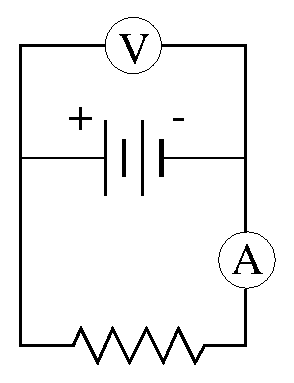
\includegraphics[scale=0.7]{2_dc/procintresist.eps}
\caption{Internal resistance measurement.}
\label{fig:DC:procintresist}
\end{figure}
\begin{table}[htb]
\begin{center}
\begin{tabular}{|c|c|}
\hline
\multicolumn{2}{|c|}{Dry cell}\\
\hline
I & V \\
\hline
\hspace*{5cm} & \hspace*{5cm} \\
& \\
\hline
& \\
& \\
\hline
& \\
& \\
\hline
& \\
& \\
\hline
& \\
& \\
\hline
& \\
& \\
\hline
& \\
& \\
\hline
& \\
& \\
\hline
& \\
& \\
\hline
& \\
& \\
\hline
\end{tabular}
\end{center}
\caption{V versus I for a dry cell.}
\label{tab:DC:DryCell}
\end{table}
\clearpage

\subsection{In-Lab Computer Work}
Plot the voltage versus the current and obtain the slope and intercept of a
curve fit1 to the plot.  Once again each student needs individual printouts. 
\begin{table}[htb]
\begin{center}
\begin{tabular}{|c|c|}
\hline
\multicolumn{2}{|c|}{Dry cell} \\
\hline
Slope & Intercept \\
\hline
\hspace*{5cm} & \hspace*{5cm} \\
& \\
\hline
\end{tabular}
\end{center}
\caption{Slope and Intercept for the dry cell $V$ vs.\ $I$ plot.}
\end{table}

\subsection{Part II Pre-Classroom Check List}
\noindent This check list is intended to be a guide for 
you to prepare yourself 
for the classroom work.  You cannot come back to lab during this hour,
collaborate with colleagues, nor hand in the worksheet late.  Make sure
you have completed everything.  
\vskip \baselineskip
\noindent {\bf Pre-classroom Check List}  
\vskip\baselineskip
\noindent $\bigcirc$ \hspace*{1cm} Table~\ref{tab:DC:newres} completed with units and uncertainties \\
$\bigcirc$ \hspace*{1cm} Table~\ref{tab:DC:lightbulb} completed with units and uncertainties \\
$\bigcirc$ \hspace*{1cm} Table~\ref{tab:DC:resistor} completed with units and uncertainties \\
$\bigcirc$ \hspace*{1cm} Table~\ref{tab:DC:DryCell} completed with units and uncertainties \\
$\bigcirc$ \hspace*{1cm} 3 Plots labeled completely and correctly \\
$\bigcirc$ \hspace*{1cm} Each student has her/his own plots and worksheet \\



\subsection{In-Classroom Calculations \& Analysis}
\noindent The following are not yes/no 
types of questions; provide the reasoning that leads you to your answer. Make 
sure that you explain clearly how particular features of the graphs are 
relevant to the answers to these questions.  

\subsubsection{Temperature Dependence of Resistance}
\noindent What does the slope of a line from the origin to a point on your graph measure? (Use Ohm's law to
determine this.) \\
\ \\
\vskip\baselineskip
\vskip\baselineskip
\vskip\baselineskip
\noindent What does the graph for the bulb measurements tell you about the
temperature dependence of resistance? \\
\ \\
\vskip\baselineskip
\vskip\baselineskip
\vskip\baselineskip
\vskip\baselineskip
\noindent What does this experiment (including the graphs) teach you about
measuring the resistance of a conductor? (the light bulb filament is a
conductor.) \\
\vskip\baselineskip
\vskip\baselineskip
\noindent Is the method of determining resistance from the slope of a $V$ vs $I$ plot preferable to using the color code or the ohmmeter? Justify your answer in any way you think. \\
\vspace*{3cm}


\noindent Use the slope you obtained from the curve fit1 to determine the value
for the resistance of the resistor.\\
\vspace*{2mm}
$$R=\mbox{\hspace*{3cm}}$$
\vspace*{1mm}\\

\noindent With the two resistance measurements from $\S$~\ref{sec:DC:tdep}, you now
have two experimental values and one nominal for the resistance of your resistor. 
What is the average and standard deviation of the three measurements? \\
\vspace*{1.5cm} \\
\vskip\baselineskip
\vskip\baselineskip

\noindent Is the relative uncertainty in the average smaller than that in the individual 
measurements? Does this make sense?\\
\ \\

\vskip\baselineskip
\vskip\baselineskip
\vskip\baselineskip
\vskip\baselineskip
\subsubsection{Internal Resistance of a Dry Cell}
\noindent What does the $V$-intercept of the graph measure? \\
\vspace*{1cm}\\
\noindent What is the internal resistance, $r$, of the battery? \\
\vfill 
$$r=\mbox{\hspace*{3cm}}$$
\noindent Attach plots to the worksheet. \\
\ \\
{\Large End Part II Worksheet} 
 


% Go back to ordinary section numbering
\renewcommand{\thesection}{\thechapter.\arabic{section}}














